\subsection{Xây dựng hệ thống}

\subsubsection{Xây dựng Dashboard}
\begin{enumerate}
    \item \textbf{Khảo sát thông tin của những người tham gia thực hiện khảo sát}\\
    Dashboard thể hiện tổng quan nhất về những người tham gia thực hiện khảo sát này với các yếu tố như độ tuổi, giới tính, trình độ học vấn, thu nhập,... thông qua
    \begin{itemize}[label=$-$]
        \item Cart thể hiện tổng số người tham gia và tất cả các khu vực.
        \item Slicer theo các thuộc tính age, state, year, fmonth để có thể linh hoạt lọc ra các thông tin theo mong muốn.
        \item Một số biểu đồ như Pie chart, Donut chart, map, treemap,...
    \end{itemize}
    \begin{center}
        \begin{figure}[!h]
            \centering
            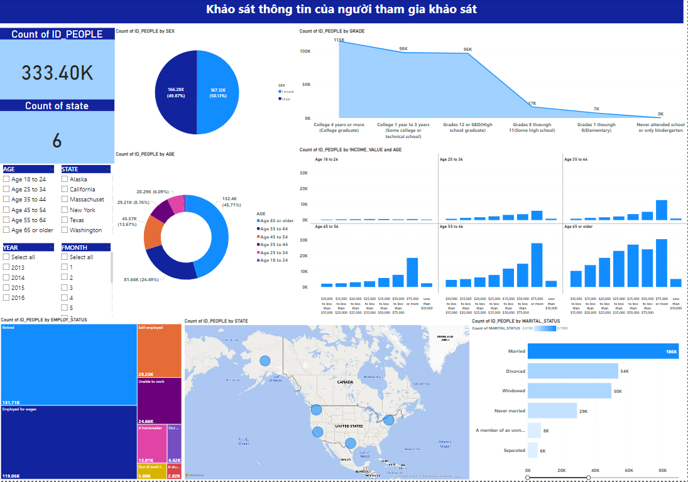
\includegraphics[scale = 0.8]{trang/dashboard1.png}
          \caption{Khảo sát thông tin của những người tham gia thực hiện khảo sát}
        \end{figure}
    \end{center}
    Từ Dashboard này ta có được thông tin phân tích như sau
    \begin{itemize}[label = $-$]
        \item Có tổng cộng tất cả là 333.4 nghìn người tham gia thực hiện khảo sát đến từ 6 bang được phân thành 6 nhóm tuổi chính từ 18 đến 24 tuổi, từ 25 đến 34 tuổi, từ 35 đến 44, từ 45 đến 54, từ 55 đến 64 tuổi và từ 65 tuổi trở lên.
        
        \item Về giới tính của người tham gia khảo sát thì tỷ lệ giữa nam và nữ là xấp xỉ nhau với nữ là 50,13\% và nam là 49,87\%.
        
        \item Về độ tuổi thì ta thấy nhóm tuổi tham gia thực hiện nhiều nhất là từ 65 tuổi trở lên chiếm 45,71\% trên tổng tất cả các nhóm tuổi, tiếp đến là nhóm từ 55 đến 64 tuổi chiếm 24,49\% và tỷ lệ này có xu hướng giảm dần theo độ tuổi, thấp nhất là nhóm từ 18 đến 24 tuổi với 1,28\%.
        
        \item Về trình độ học vấn thì số người đã tốt nghiệp cao đẳng,đại học đa số chiếm phần lớn và xếp sa lần lượt là đang học cao đẳng, đại học và tốt nghiệp lớp 12.
        
        \item Về thu nhập thì ở nhóm tuổi từ 18 đến 24 tuổi mức thu nhập được trải đều còn với các nhóm tuổi còn lại thì mức thu nhập hầu hết là hơn \$ 75000, riêng với nhóm từ 65 tuổi trở lên thì tỷ lệ mức thu nhập từ dưới \$ 75000 nhiều hơn so với các bảng còn lại.
        
        \item Về tình trạng việc làm vì chủ yếu người tham gia khảo sát là trên 65 tuổi nên đa số đã về hưu, theo sau đó là những người làm công ăn lương cũng chiếm khá đông.
        
        \item Về số lượng người tham gia thực hiện theo vị trí địa lý ta thấy tỷ lệ người tham gia từ các bang là tương đương nhau.
        
        \item Về tình trạng hôn nhân thì chủ yếu là những người đã kết hôn với hơn 186 nghìn người trên tổng số hơn 333 nghìn người chiếm hơn 50\%.
    \end{itemize}
Qua đó, ta thấy khảo sát này được thực hiện đa số ở những người trung tuổi nên hầu hết đã có việc làm hoặc đã về hưu và tuy họ ở các khu vực khác nhau nhưng đời sống đều ở mức ổn định.
    
    \item \textbf{Khảo sát về khả năng tiếp cận y tế}\\
    Khả năng tiếp cận y tế tùy thuộc vào hoàn cảnh của mỗi người nên việc xây dựng Dashboard này để thể hiện các vấn đề về việc khám sức khỏe với 
    \begin{itemize}[label=$-$]
        \item Cart thể hiện tổng số người tham gia và tất cả các khu vực.
        \item Slicer theo các thuộc tính age, state, year, fmonth để có thể linh hoạt lọc ra các thông tin theo mong muốn.
        \item Một số biểu đồ như Pie chart, Donut chart, Area chart, 100\% Stacked column chart,...
    \end{itemize}
    \begin{center}
            \begin{figure}[!h]
                \centering
                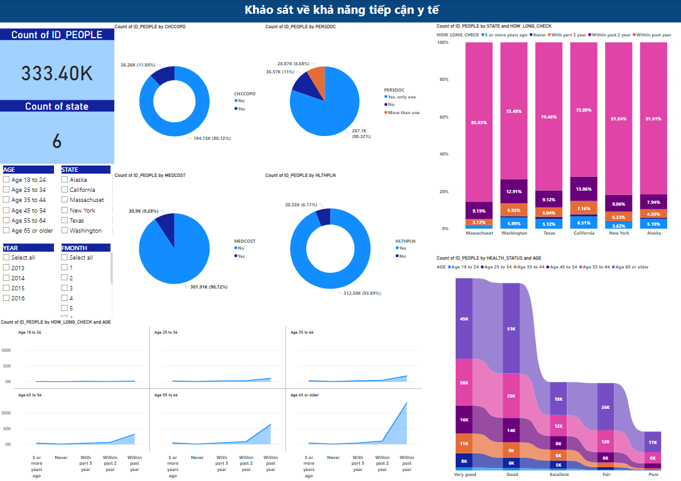
\includegraphics[scale = 0.8]{trang/dashboad2.png}
              \caption{Khảo sát về khả năng tiếp cận y tế}
            \end{figure}
\end{center}
    \newpage
    Từ Dashboard này ta có được thông tin phân tích như sau
    \begin{itemize}[label=$-$]
        \item Tỷ lệ người từng mắc bệnh tắc nghẽn phổi mãn tính là 11,88\%.
        
        \item Số người có bác sĩ riêng chiếm khá ca trong đó có đến 80,32\% là có một bác sĩ riêng và 8,68\% là nhiều hơn một bác sĩ.
        
        \item Trong đó cũng có những người chưa có đủ điều kiện đi thăm khám bác sĩ cần thiết trong vòng 12 tháng qua chiếm 9,28\%.
        
        \item Số người tham gia bảo hiểm y tế rất cao chiếm gần 94\%.
        
        \item Về lần cuối đi khám sức khỏe, ta thấy mọi người thường xuyên đi khám sức khỏe và nhóm từ 65 tuổi trở lên có tỷ lệ đi khám sức khỏe lớn nhất do càng lớn tuổi thì sẽ càng quan tâm chăm sóc sức khỏe nhiều hơn, ngược lại nhóm từ 18 đến 24 tuổi chiếm tỷ lệ thấp nhất.
        
        \item Xét về từng khu vực thì thấy Massachuset có tỷ lệ thăm khám đều đặn hơn so với các khu vực còn lại.
        
        \item Về tình trạng sức khỏe theo độ tuổi thì từ 18 đến 24 tuổi trạng thái tốt hơn hẳn, từ 25 đến 64 tuổi có sức khỏe tốt chiếm phần lớn và trên 65 tuổi trở lên số người có tình trạng không ổn chiếm nhiều hơn so với các nhóm tuổi khác, đó cũng là điều dễ hiểu.
    \end{itemize}
 Qua đó, ta thấy về chất lượng cuộc của những người này khá ổn với đa số người có bác sĩ riêng và có tham gia bảo hiểm y tế, về việc đi khám sức khỏe cũng được diễn ra thường xuyên.
    
    \item \textbf{Khảo sát về tình trạng hút thuốc lá}\\
    Dashboard thể hiện tình trạng hút thuốc lá theo các yếu tố như độ tuổi, tần suất sử dụng,...  
    \begin{itemize}[label=$-$]
        \item Slicer theo các thuộc tính age, state, fmonth để có thể linh hoạt lọc ra các thông tin theo mong muốn.
        \item Một số biểu đồ như Pie chart, Donut chart, Area chart, Clustered column chart,...
    \end{itemize}
    \begin{center}
            \begin{figure}[!h]
                \centering
                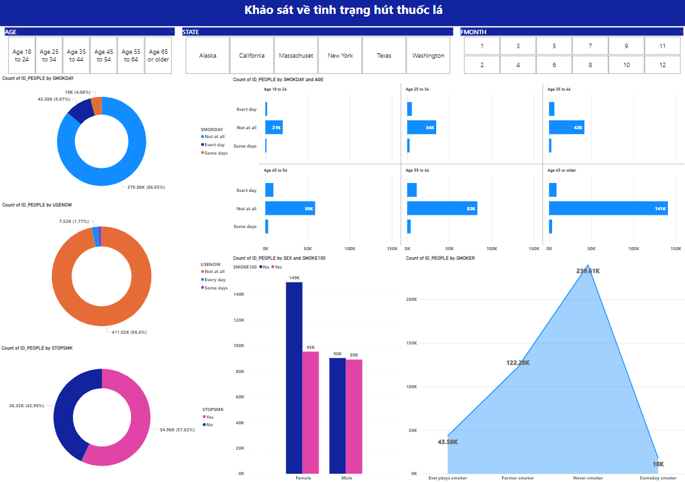
\includegraphics[scale = 0.8]{trang/dashboard3.png}
              \caption{Khảo sát về tình trạng hút thuốc lá}
            \end{figure}
    \end{center}
    Từ Dashboard này ta có được thông tin phân tích như sau
    \begin{itemize}[label= $-$]
        \item Số lượng người hút thuốc mỗi ngày chiếm 9,87\% còn lại là số lượng người chưa hút thuốc hoặc hút ít.
        
        \item Thói quen hút thuốc theo nhóm tuổi: số lượng người hút thuốc mỗi ngày ở nhóm từ 45 đến 54 tuổi và từ 55 đến 64 tuổi là đông hơn so với các nhóm còn lại.
        
        \item Số lượng người cố gắng bỏ thuốc chiếm 57,02\% so với những người chưa có ý định đó.
        
        \item Ở nữ thì việc hút ít hơn 100 điếu có số lượng nhiều hơn hắn so với việc hút nhiều hơn 100 điếu. Còn ở nam thì việc hút ít hơn hay nhiều hơn 100 điếu là ngang nhau và ngang với số người nữ hút nhiều hơn 100 điếu.
        
        \item Cuối cùng là số lượng người hút thuốc theo tấn suất thì ở đây ngoài việc không sử dụng là chủ yếu thì tiếp đến là người đã từng sử dụng chiếm khoảng $\frac{1}{3}$ tổng người tham gia, sau đó mới đến người hút hàng ngày và hút ít.
    \end{itemize}
    Qua đó, ta thấy trong những người tham gia thực hiện khảo sát này thì số người sử dụng thuốc lá là không nhiều.
\end{enumerate}

\subsubsection{Bài học tổng kết}
Sau khi cùng nhau tìm hiểu và hoàn thành bài tập nhóm này, nhóm chúng em đã rút ra được một số bài học như sau
\begin{enumerate}
    \item Cần tìm hiểu kĩ về chuyên môn, nghiệp vụ và các quá trình liên quan trước khi phân tích thiết kế và xây dựng Datawarehouse

    \item Kích thước dữ liệu lớn cần phải import và ETL sao cho hợp lý
    
    \item Dữ liệu trong thực tế không bao giờ hoàn hảo, luôn có các trường cần xử lý
    
    \item Data model phải có quan hệ giữa các bảng, thông tin như khoá chính, kiểu dữ liệu,...
    
    \item Dashboard phải bám sát nghiệp vụ, đảm bảo tính đa dạng, trực quan, có các thành phần như: footer, header, slicer,...
    
    \item Dashboard phải mang tính phân tích, so sánh, không quá tập trung vào thống kê, miêu tả.
\end{enumerate}


